The Spot Trace data from the Timor Sea and Arafura Sea fisheries illustrate a classic "fishing the line" phenomenon. Many vessels fish right at the Indonesia - Australia border, on the edge of better managed fishing grounds on the Australian side, where fish densities are expected to be higher. Several drop line fishers were observed to operate illegally in Australian waters and some of these have been arrested by Australian patrol boats in 2015. Some drop line long line vessels have also been observed to illegally fish in Timor Leste waters. There is apparently little or no enforcement of fisheries regulations in Timor Leste waters and especially the Joint Petroleum Development Area or JPDA (an area in Timor Leste waters where a resource sharing agreement for seabed resources is in place with Australia) is frequently targeted illegally by Indonesian vessels.

The Spot Trace data from WPP 718 and surrounding areas show great mobility of the medium-scale snapper fishing boats, making trips to fishing grounds that are up to 1,000 kilometers away from home ports. Not only are these fleets highly mobile in terms of their trips from home port, they are also flexible in changing their base of operations from one port to another, changing from landing at home port to offloading on transport vessels in remote ports or offloading for air cargo at yet other places. Decision making on movements by boat owners can be based on fisheries technical issues such as catch rates or weather, but also on administrative issues like licensing or enforcement of rules against under-marking in Gross Tonnage. Most recently we are observing movement of staging ports but also of processing capacity to remote areas in the east such as the island of Penambulai, East of the Aru Islands. Fish is landed there and moved onto transport vessels bound for processing plants elsewhere in the country.

Therefore the fish that is processed in major processing centers like Probolinggo comes from a number of different fleets that operate throughout the waters of Eastern Indonesian, including also WPP 718. For the purpose of this report, all fishing trips, recorded (from SPOT data) within WPP 718, mostly from long line and drop line operations, were included in the analysis for this WPP. This includes fishing trips originating from outside the WPP, for example from Probolinggo, Bali or Kema.

Potential IUU issues include the operation by various fleets outside Indonesian waters in the East Timorese - Australian JPDA as well as in strictly Australian waters. Additional issues include the under marking of medium scale vessels to below 30GT, the licensing of the various fleets for various WPP and the operation of fleets from remote ports inside Marine Protected Areas throughout Eastern Indonesia. All this needs to be discussed with fishing boat captains and boat owners to prevent issues of supply line "pollution" with IUU fish from thee protected areas.

\begin{center}
\graphicspath{{/root/R-project/IFishSnapperWPP718/Images/}}
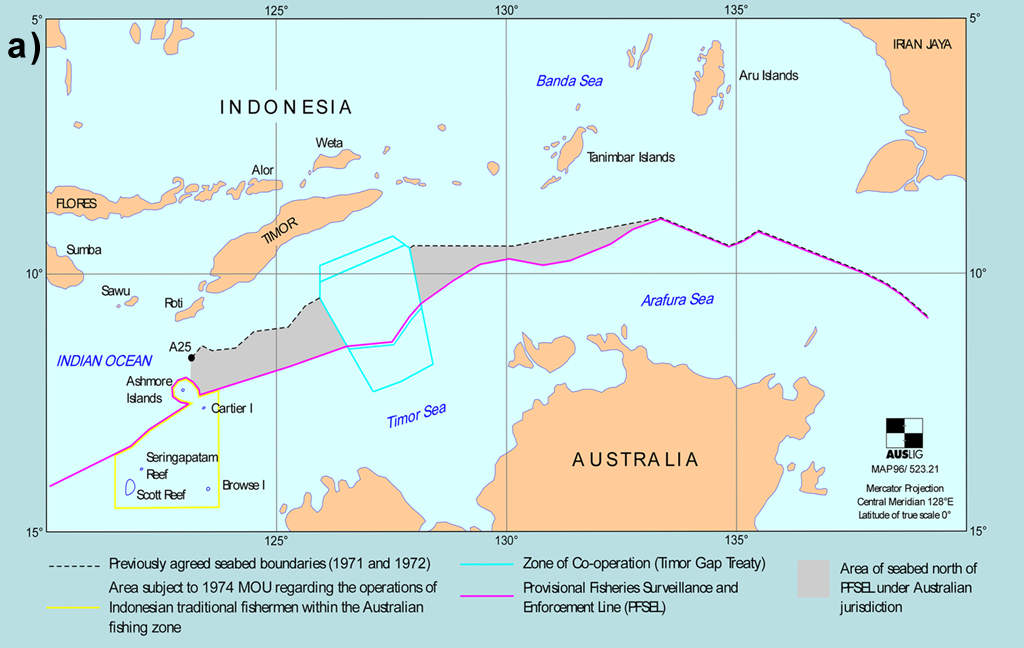
\includegraphics[scale=0.4]{JPDA-Map.png}
\end{center}

\begin{wrapfigure}{r}{8cm}
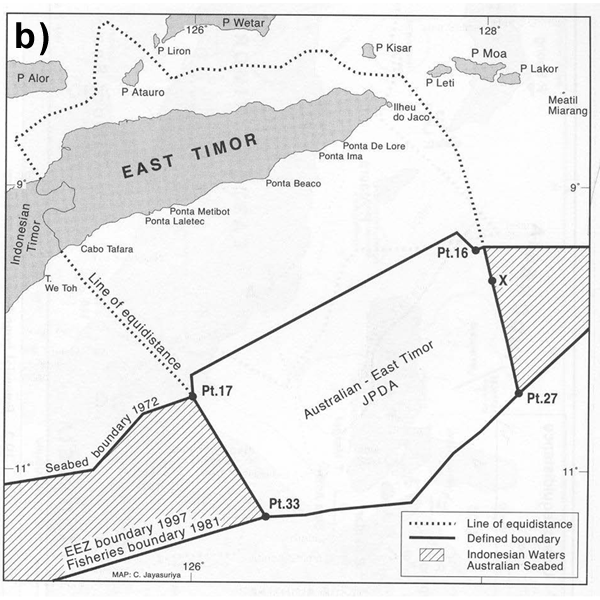
\includegraphics[width=1\linewidth]{/root/R-project/IFishSnapperWPP718/Images/JPDA-Map-bw.png}
\end{wrapfigure}

Figure 5. Timor Sea and Arafura Sea fishing grounds with current boundaries between Indonesia, East Timor and Australia.

a) The dotted line is the Australia - Indonesia Seabed Boundary. The pink line (PFSEL) is the Australia - Indonesia Fisheries Boundary. Indonesian vessels are allowed to fish in the grey area between the pink line and the dotted line, but not below the PFSEL. The light blue line is the boundary of the East Timor - Australia Zone of Cooperation which covers East Timorese fishing grounds where Indonesian fishing vessels are not allowed to fish. Australia does not enforce fisheries regulations here.

b) The shaded area between the Seabed Boundary and the Fisheries Boundary is Australian seabed, where fishers from Indonesia are allowed to fish. The Australian - East Timor zone of cooperation or �Joint Petroleum Development Area� (JPDA) is not open to fishers from Indonesia. East Timor is responsible for fishery surveillance within the JPDA.

Source: Australian Surveying \& Land Information Group (AUSLIG) Commonwealth Department of Industry Science and Resources. MAP 96/523.21.1.

\clearpage
\newpage

\begin{center}
\graphicspath{{/root/R-project/IFishSnapperWPP718/Images/}}
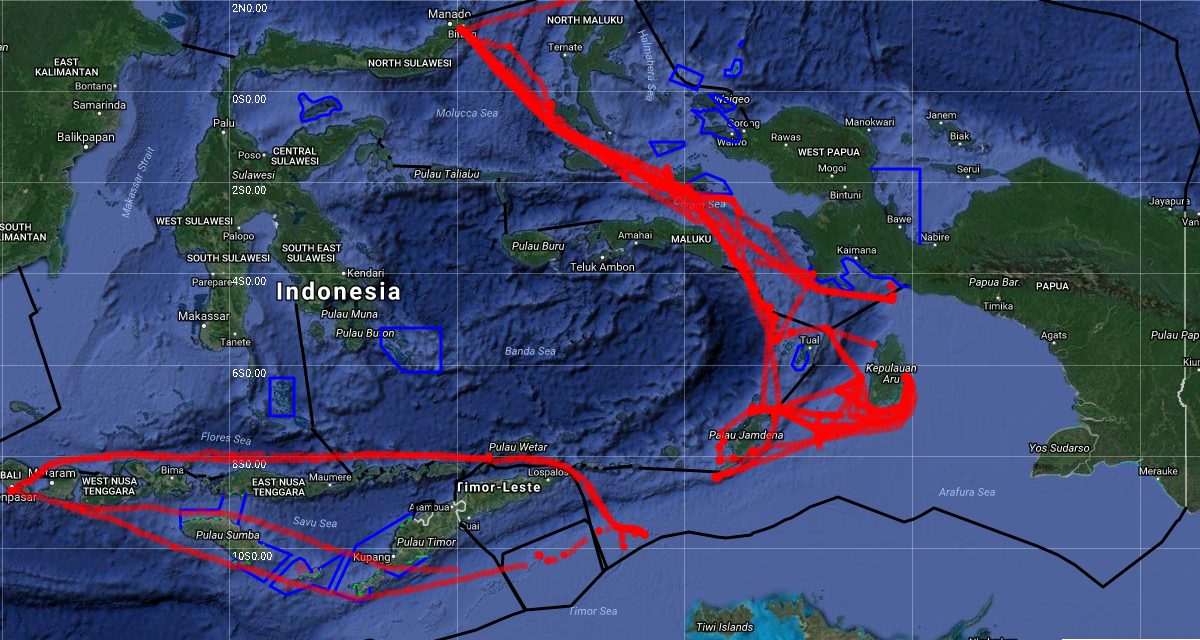
\includegraphics[width=15cm]{SpotTrace-AreaD-Dropline.png}

Figure 6. Tracks of drop line fishing boats from various ports, operating in the Arafura Sea (WPP 718) and the JPDA (East Timor waters).
\end{center}

\begin{center}
\graphicspath{{/root/R-project/IFishSnapperWPP718/Images/}}
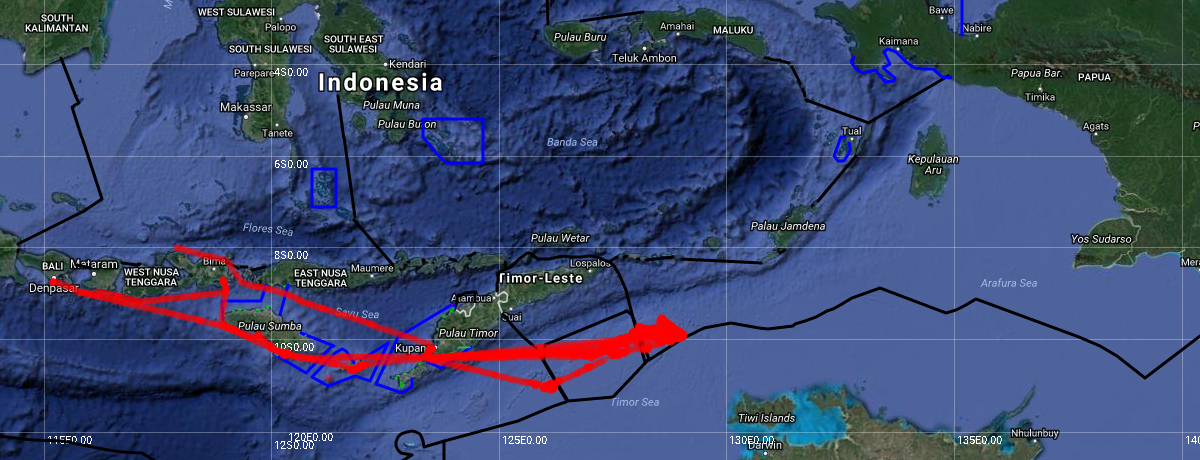
\includegraphics[width=15cm]{SpotTrace-AreaD-Longline.png}

Figure 7. Tracks of bottom long line fishing boats from various ports, operating in the Arafura Sea (WPP 718) and the JPDA (East Timor waters)
\end{center}